\section{Structural Analysis}

\label{sec:structural}

Structural analysis studies the interrelation between parameters and variables of the system using constraints between them. It distinguishes known and unknown variables, according to whether they can be measured in the system or not. Then the unknown variables are expressed using the known ones according to the constraints. Structural analysis based residual signal require that unknown variables can be expressed redundantly. One of the constraints is used to express the unknown, the other to verify it. If there's a mismatch between the two, a fault is detected.

In case of fault detection in sensors, one constraint is between the measured and the actual values of a variable. In case of a sensor fault, there can be a considerable difference between the measured and the actual value of a variable. Assumes that only one fault occurs at any given time, so faults cannot mutually neutralize each other. 

The constraints being used to detect faults in the motor are \ref{sec:motor} \todo{reference motor section properly}


\begin{equation}
V_a = R_a i + k_e \omega
\end{equation}

\begin{equation}
 k_{t}i  =J\dfrac{d\omega}{dt} + b\omega
\end{equation}

\begin{equation}
\tau = k_t i
\end{equation}

\begin{equation}
d_1(\omega, \dot{\omega})
\end{equation}

$\omega$ and $i$ can be measured, so the residual signal can be derived as


\begin{equation}
residual = k_t i + J \frac{d\omega}{dt} + b \omega
\end{equation}

The fraction model is quite accurate at high speeds, not so much for low speeds. This needs to be addressed by a higher threshold at low speeds.

\begin{figure}[h]
	\centering
	\begin{tabular}{@{}c@{\hspace{.5cm}}c@{}}
		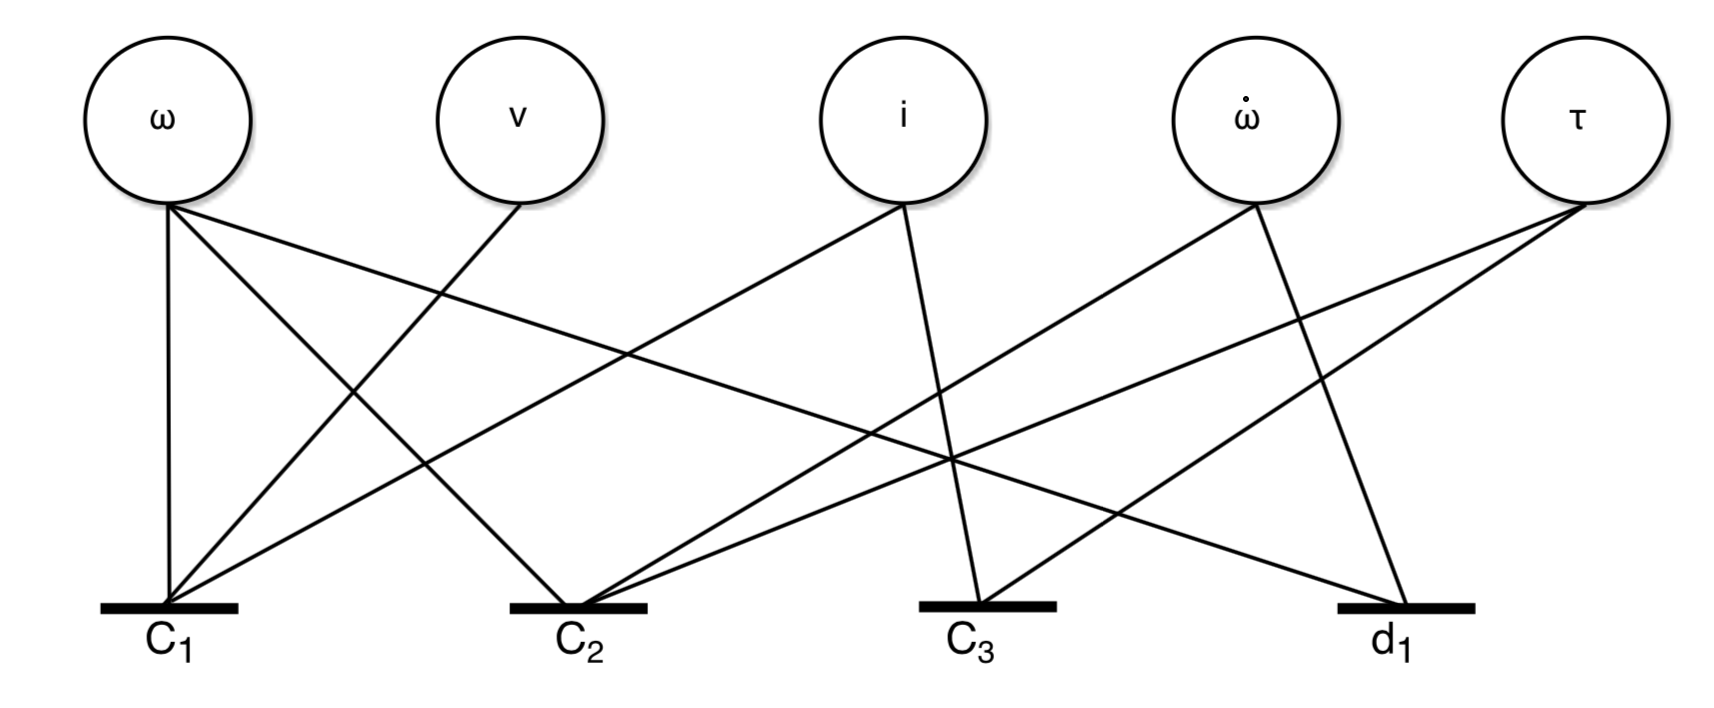
\includegraphics[page=1,width=1\textwidth]{fault_diagram}
	\end{tabular}
	\caption{Structural graph of reaction wheel motor}
	\label{fig:CascadeDesat}
\end{figure}



